% Remember to input this to the presentative tex file before compiling.
\chapter{Related Work}

\tab There exists a number of challenges in predicting trajectories in the context of self-driving cars. One of those crucial factors is behavior of pedestrians. Due to their ability to move around freely and cross the streets in the same environment as AV, it is important that their safety is ensured by the self-driving cars, irrespective of pedestrians' actions \cite{fragkedaki2024pedestrianmotionpredictionusing}. Because of their "large degree of freedom" \cite{fragkedaki2024pedestrianmotionpredictionusing}, it becomes challenging to model their behavior in a dataset. Therefore other largely available datasets don't provide information for autonomous cars to understand the intention of other traffic agents \cite{rasouli2017ICCVW}. Studies, such as those by Rasouli et al.\cite{rasouli2017ICCVW}, emphasize that pedestrians often engage in non-verbal communication, such as eye contact or gestures, which can significantly influence traffic flow and the decisions made by AV systems. To this end, in their paper "Are they going to Cross?" \cite{rasouli2017ICCVW}, Rasouli et al. introduced a new dataset, Joint Attention in Autonomous Driving (JAAD), which provides not only bounding box information for object detection, but also is annotated with behaviour and contextual details of those present in the traffic scenes. Figure \ref{fig:jaad1} gives an example of the annotations provided by JAAD dataset. 


\begin{figure}[h]
  \begin{center}
     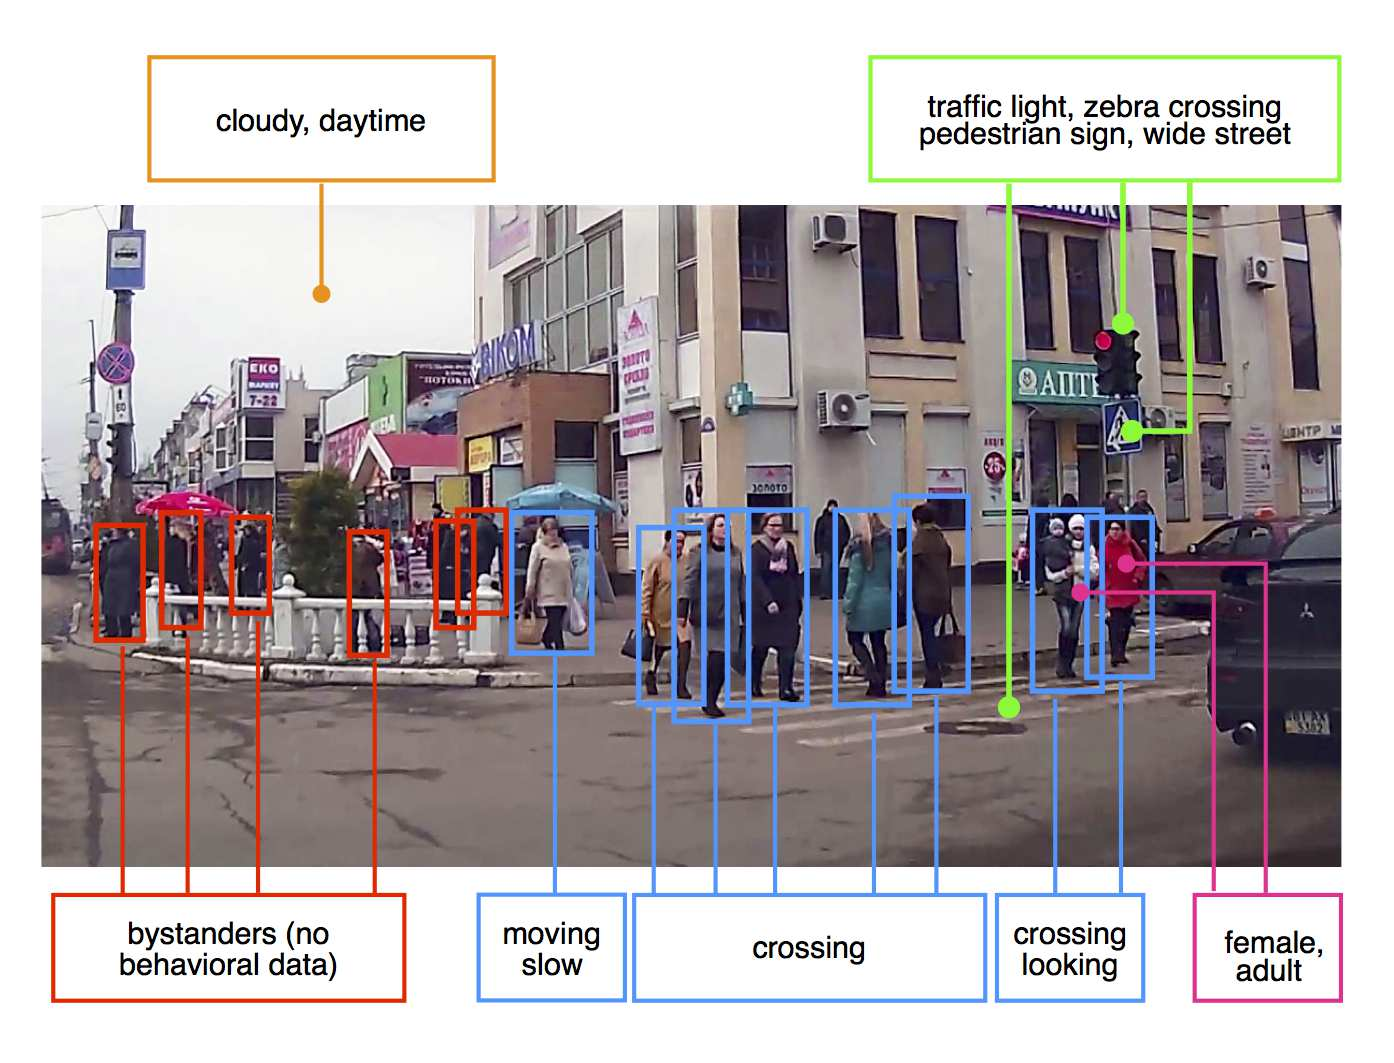
\includegraphics[height=90mm]{Images/Figures/jaad_fig1.png}
  \end{center}
  \caption{JAAD annotations with bounding boxes for all pedestrians, behavioral labels and contextual tags}
  \label{fig:jaad1}
\end{figure}

\tab JAAD dataset particularly focuses on numerous crossing scenarios for pedestrians as the authors of the paper consider most of the interaction with the driving cars to happen at the crossing points \cite{rasouli2017ICCVW}. Their dataset includes three types of ground truth annotations: bounding boxes of pedestrians for object detection, behavioral tags for denoting pedestrians' states and scene annotations for environmental contextual elements. The behavioral information includes the type and duration of pedestrians' actions, as well as the actions of the driver. Pedestrians' actions are divided into three categories: Precondition - pedestrians' state before crossing (i.e., standing, moving slowly, or fast), Attention - pedestrians' awareness towards approaching vehicle , looking for more than 1 second or glancing for less than 1 second, and Response - actions of the pedestrians after being aware of the approaching vehicle. This includes responses such as stopping, clearing the path, slowing down, speeding up, hand gestures, or nodding in reaction to the vehicle. Additionally, complementary tags come with demographics of the pedestrians like gender, age (adult, child, elderly), and group size.
Figure \ref{fig:jaad2} describes an example of behavioral labelling. 


\begin{figure}[h]
  \begin{center}
     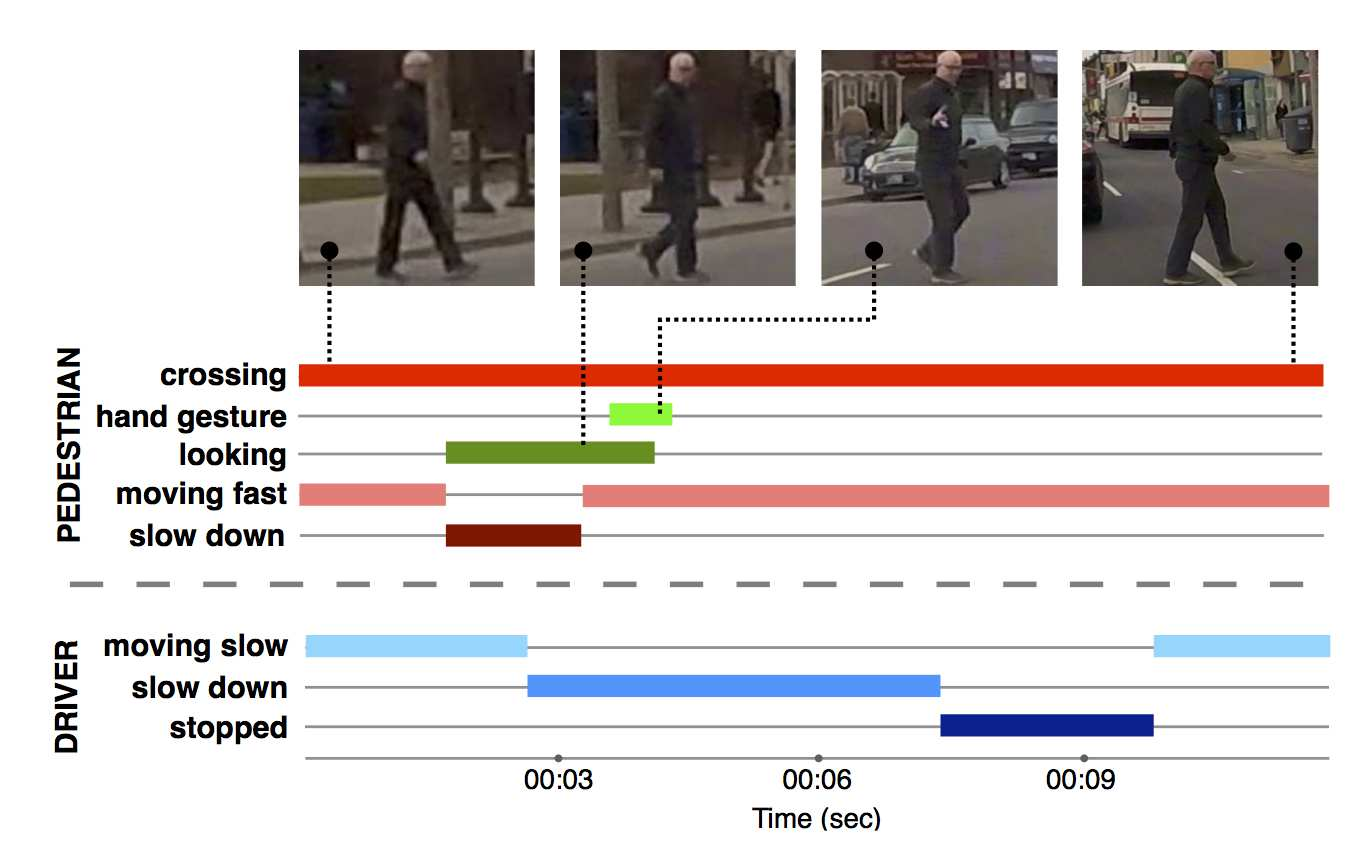
\includegraphics[height=90mm]{Images/Figures/jaad_fig2.png}
  \end{center}
  \caption{JAAD behavioral annotations with timestamps at a crossing point}
  \label{fig:jaad2}
\end{figure}

\tab Another crucial factor in AV system and subsequently for trajectory prediction is to get enhanced information about the driving environment, such as crosswalks, sidewalks, drivable areas and other contextually essential features, that is needed to make informed decisions from the side of AV.  The segmentation process assigns semantic labels to each pixel in an image, distinguishing between different object types and scene elements \cite{sun2024semanticformerholisticsemantictraffic}. Semantics segmentation helps to improve the safety of AV's operation by outlining drivable area and lane markings \cite{che2024twinlitenetplusstrongermodelrealtime}. Deep neural networks employ encoder-decoder structures or spatial pyramid pooling modules to perform semantic segmentation tasks \cite{DBLP:journals/corr/abs-1802-02611}. Encoder-decoder capture sharper object boundaries and gradually recovers the spatial information whereas spatial pyramid pooling encodes multi-scale contextual information by probing the incoming features with filters or pooling operations at multiple rates and multiple effective fields-of-view \cite{DBLP:journals/corr/abs-1802-02611}. DeepLabV3+ \cite{DBLP:journals/corr/abs-1802-02611} combines both these methods that allows them to achieve refined segmentation results along object boundaries. Figure \ref{fig:deeplab} shows the application of DeepLabV3+ on Cityscapes dataset.


\begin{figure}[h]
  \begin{center}
     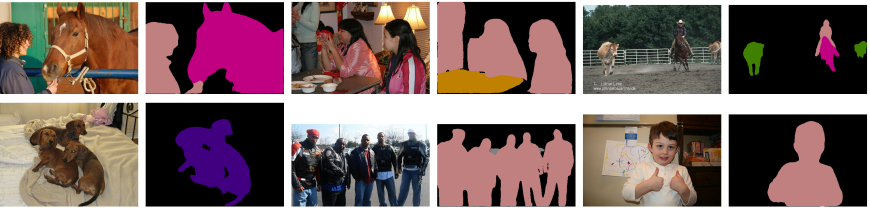
\includegraphics[scale=0.5]{Images/Figures/deeplabv3+.png}
  \end{center}
  \caption{Semantics Segmentation of DeepLabV3+ on Cityscapes dataset}
  \label{fig:deeplab}
\end{figure}

\tab Yet another component required in an AV system is object detection. This process involves locating and categorizing objects \cite{silva2024recurrentyolov8basedframeworkeventbased} within an image or a video frame. Development in the field has been made commonly with the use of Deep learning algorithms such as You Only Look Once (YOLO) detectors that is based on Convolutional Neural Network(CNN) \cite{silva2024recurrentyolov8basedframeworkeventbased}. YOLO is able to perform object detection in real-time, with a fast speed and great accuracy \cite{yolov3}. For this reason, YOLO was later applied on the dataset for safe navigation of autonomous vehicles in a traffic scene.

\tab Although a lot is being done for trajectory prediction on objects, only a number of them consider the importance of nearby objects \cite{2019itsc_grip}. This issue has been taken into consideration and new researches have been made that takes into account the "social interaction" \cite{10397282} between target vehicle, that which we want to predict the trajectory, and its environment that contains other traffic agents such as bicycles, cars and pedestrians. 



\tab Cui et al. \cite{8793868} proposed, focusing on multi-modality of a traffic scenario, a method to predict multiple possible trajectories of a given actor as well as estimating their probabilities. Their proposed network encodes  \(300 \times 300\) bird-eye-view raster image of a nearby traffic actor with \(0.2m\) resolution and the actor's current state, such as velocity, acceleration, heading change rate, as input and outputs \(M\) modes of future \(x-\) and \(y-\) positions. The positions are outputted with \(2H\) per mode, where \(H\) denotes the number of future consecutive time steps for which the states are predicted along with their probabilities. This overall results in \((2H + 1)M\) outputs for each actor. To ensure that the probability outputs sum up to 1, they pass the results through a softmax layer. Their method allows any CNN architecture to be used as the base network and the authors applied MobileNet-v2. 

\tab Luo et al. \cite{luo2020fastfuriousrealtime} introduced in their paper a fast detection, tracking and motion predicting of objects. Bird's eye view LiDAR data is given as input and 3D is processed spatially and temporally. Afterwards they add two branches of convolutional layers where one calculates the probability of a vehicle being at a given location and the other forecasts bounding boxes of the subsequent frames. These available approaches require high computational power if they are to perform trajectory predictions of all nearby objects in a traffic scene \cite{2019itsc_grip}. Therefore Li et al. developed a robust and more efficient object trajectory prediction scheme to forecast the accurate future positions of those objects surrounding the self-driving cars \cite{2019itsc_grip}. Moreover they further improved  their scheme \cite{li2020gripplus} and this paper utilizes the enhanced version.


\section{GRIP Scheme Description}

\tab The algorithm that will be the focus of this paper is Enhanced Graph-based Interaction-aware Trajectory Prediction (GRIP++) \cite{li2020gripplus}. It is designed to predict trajectory of traffic participants around an AV more efficiently using graph to represent interaction amongst close objects, applies multiple graph convolutional blocks to extract features and ultimately uses LSTM encoder-decoder to make predictions. This section summarizes and provides a detailed description of the scheme.

\subsection{Analysis}

\tab Most of the algorithms used in the traffic scene are limited in several ways such as one where it doesn’t work in crowded scenarios, or with the second example it merely predicts the trajectory of one specific car but since the traffic will be composed of more than one vehicle at a given time, this method becomes highly inefficient. Nonetheless these methods require intensive computation power if they want to predict the trajectory of all surrounding objects. And if they are maneuver based, wrong classification of the maneuver type will negatively impact the trajectory prediction.

\tab Li et al., formulates the problem as follows: trajectory prediction is a problem that estimates the future positions of all objects in a scene based on their trajectory histories. Therefore the inputs X of the model are trajectory histories(over \(t_h\) time steps) of all observed objects in a traffic scene:

\begin{equation}
    X = [p^{(1)}, p^{(2)},.....,p^{(t_h)}]
\end{equation}

where,

\begin{equation}
    p^{(t)} = [x_0^{(t)}, y_0^{(t)}, x_1^{(t)}, y_1^{(t)}, ... ,x_n^{(t)}, y_n^{(t)}]
\end{equation}


are the coordinates of all observed objects at time t, and n is the number of observed objects in that scenario. Their format is the same as another study done by Deo et al. and global coordinates are used. To improve the prediction accuracy, the “ego-vehicle-based” coordinate system could be used as suggested by the author but is not applied for future work. 
Because their model takes in histories of all observed objects in a traffic scenario, it was argued to be most fitting to predict the future position of all of them simultaneously rather than focusing on one individual object, which is a preferred measure for other schemes that are also predicting future position for autonomous cars. The outputs Y of the proposed model are the predicted positions of all observed objects in a scenario from time step \(t_h + 1\) to \(t_h+ t_f :\)

\begin{equation}
    Y = [p^{(t_h+1)}, p^{(t_h+2)},........., p^{(t_h+t_f)}]
\end{equation}

where \(p^{(t)}\) is the same as the second equation described above and \(t_f\) is the predicted horizon.

\tab In there proposed scheme , the authors of the paper divide their approach towards their novel model into following components: 
\begin{enumerate}
    \item Input Preprocessing Model,
    \item Graph Convolution Model
    \item Trajectory Prediction Model
    \item Implementation Details
\end{enumerate}

\subsubsection{Input Preprocessing Model}

\textbf{\textit{A. Input Representation:}} Prior to feeding the raw data into the model, it is required to convert it into a specific format for subsequent efficient computation. Given \(n\) objects in a traffic scene in the past \(t_h\) time steps, it is represented in a 3D array \(F_{input}\) with a size of \((n \times t_h \times c)\). The authors set \(c= 2\) in the paper to indicate x and y coordinates of an object. Since it is easier to predict the velocity of an object rather than predicting its location(Li et al., 2020), velocities \((p^{t+1} - p^t)\) is calculated before feeding the data into the model. 

\textbf{\textit{B. Graph Construction:}} As in an autonomous driving application scenario, the movement of a target’s surrounding objects deeply impacts the motion of the target, the authors represent the inter-object interaction using an undirected graph \(G= \{V, E\}\). Each node, \(V\) corresponds to an object present in a traffic scene. Given that each object would have different states at different time steps, the node set \(V = \{v_{it}| i=1,....,n, t =1,...t_h\}\) where \(n\) is the number of observed objects and \(t_h\) is the observed time steps. The feature vector \(v_it\) on a node is the coordinate of \(i_{th}\) object at time \(t\).

\tab In constructing the graph, objects that have interaction at each time step \(t\) are connected via edges. Authors define such interaction in an autonomous driving scenario when two objects are close to each other. Therefore the edge set \(E\) consists two parts: (a) the interaction information between two objects in spatial space time \(t\), called “spatial edge” (Li et al., 2020) and denoted as \(E_S = \{v_{it}v_{jt}|(i,j \in D)\}\), with \(D\) being a set where objects are close to each other. This is demonstrated in the Figure \ref{fig:gripscheme}, using two blue circles with a \(D_{close}\) radius on the “Raw Data” section. Objects that are inside the blue circle are regarded as close to the object located in the middle, indicated by a blue dot. Therefore in the diagram, the top object has three close neighbors whereas the one below has one neighbor. (b) The second part is the “inter-frame edges” (Li et al., 2020), that essentially represents the historical information frame by frame in temporal space. The temporal edge connects each observed object in a given time step with itself in another time step, and is denoted as \(E_F = \{v_{it}v_{i(t+1)}\}\). In such a way\(E_F\) contains all edges of a particular object which represent its trajectory over time steps. 

\tab The authors of the algorithm represent this graph using an adjacency matrix \(A = \{A_0, A_1\}\),  where \(A_0\), an identity matrix \(I\), represents self-connections and \(A_1\), an adjacency matrix, represents spatial connection, for more efficient computation. At a given time \(t\),


\begin{equation}
    A_0[i][j] (or A_1[i][j]) = 
    \begin{cases}
        1, & \text{if edge} {0.5mm} \langle v_{it}, v_{jt}\rangle  \in E\\
        0, & \text{otherwise}
    \end{cases}
\end{equation}

\(A_0\) and \(A_1\) both are of size (\(n \times n\)), where \(n\) is the number of observed objects in a traffic scene. The authors called it “Fixed Graph” as  it is constructed on a manual design rule and is fixed once the input data is given and will not modify during the training phase. It is shown in Figure \ref{fig:gripscheme} as a blue dots connected graph symbol. 

\begin{figure}[h]
  \begin{center}
     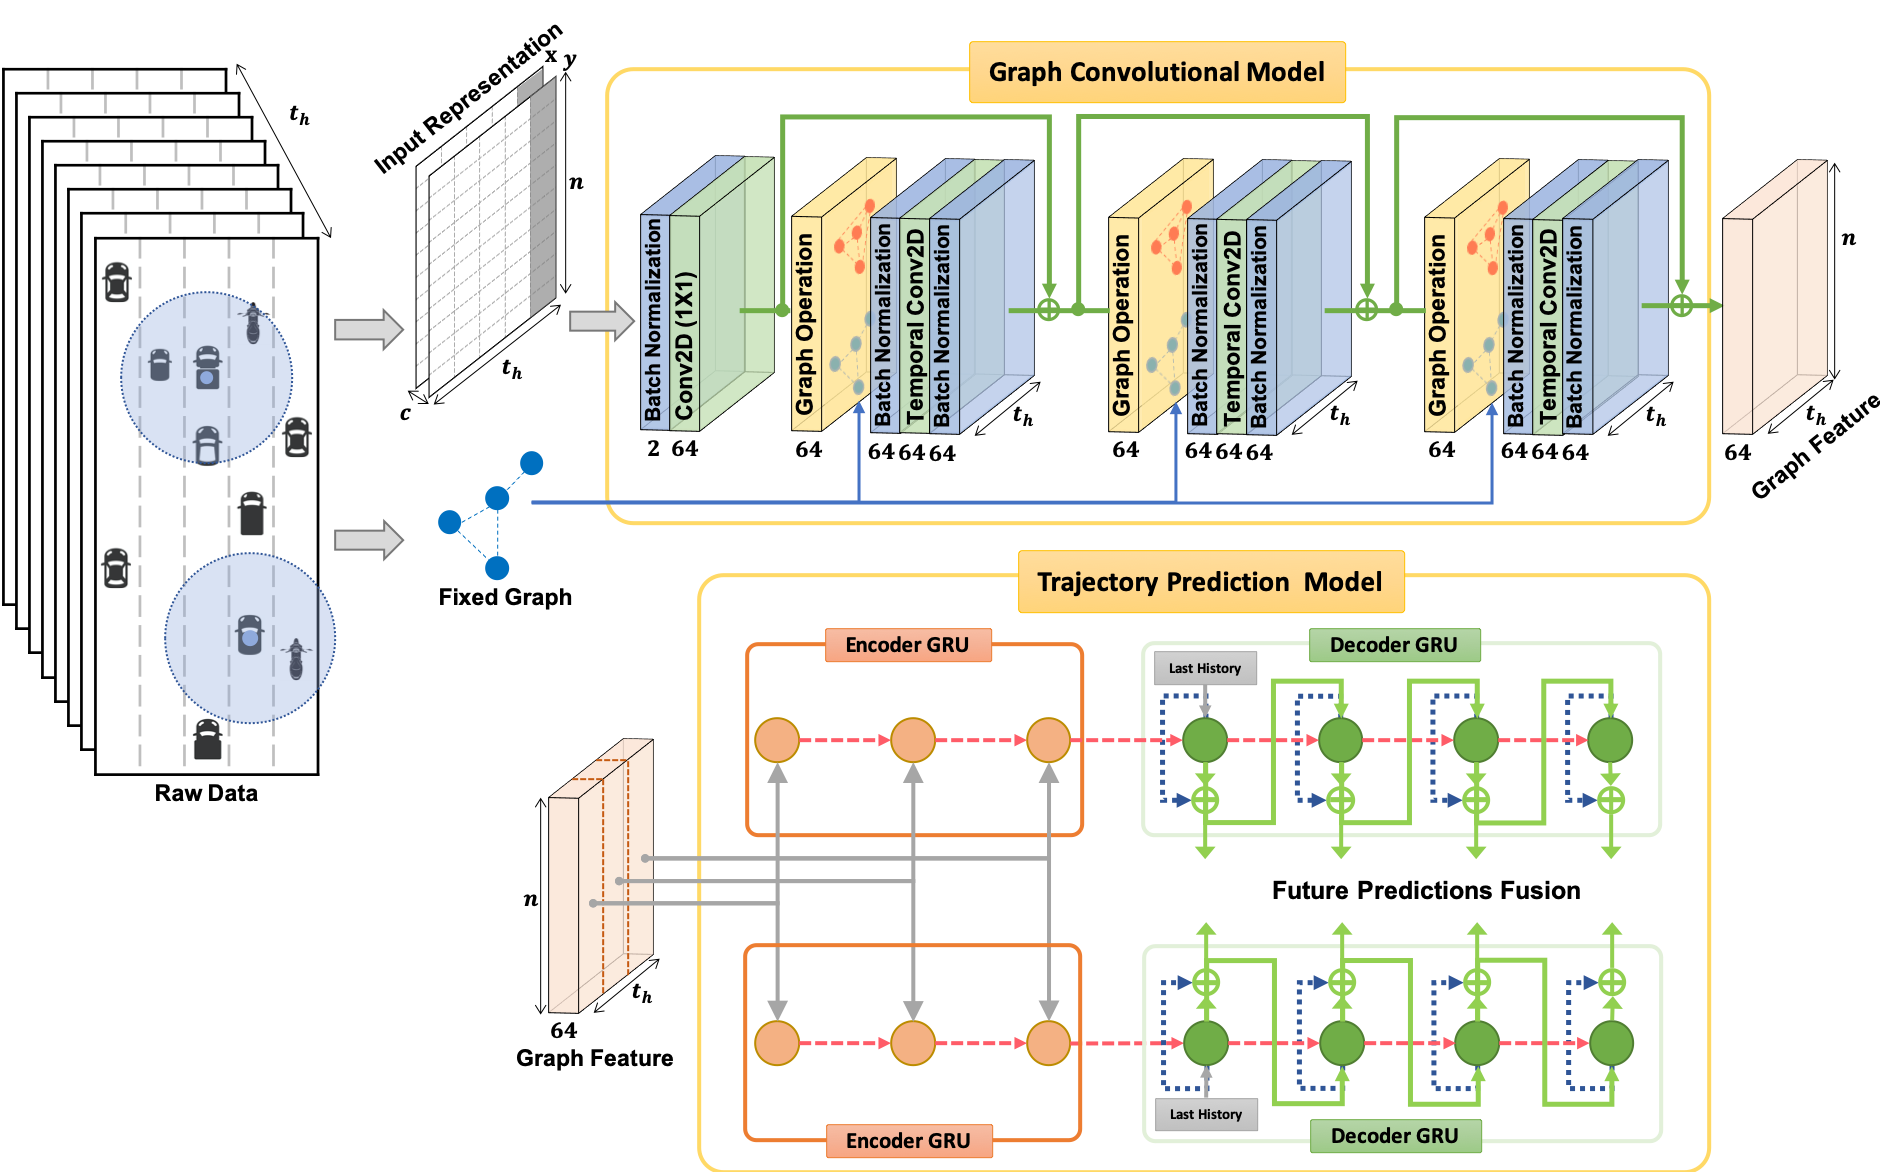
\includegraphics[height=90mm]{Images/Figures/figure1.png}
  \end{center}
  \caption{GRIP++ proposed Scheme}
  \label{fig:gripscheme}
\end{figure}

\subsubsection{Graph Convolutional Model}

\tab For a given preprocessed input data \(F_{input} := \mathbb{R}^{n \times t_h \times c}\), the Graph Convolutional Model passes it through a 2D convolutional layer with \((1 \times 1)\) kernel size, shown in Figure \ref{fig:gripscheme} as "Conv2D \((1 \times 1)\)", so that the number of channel is increased. It is designed to map the 2 dimensional input data (x and y coordinates) into a higher dimensional space to help the model learn a good representation for the trajectory prediction task. The output, therefore, is of the shape \((n \times t_h \times C)\), where \(C\) is the new number of channels. In the figure \ref{fig:gripscheme}, \(C\) is 64. The input data is then fed into both several graph operations and temporal convolutions where graph operations handle the inter-object interaction in spatial space and temporal convolutions capture useful temporal features such as motion pattern of an object. Therefore, Figure \ref{fig:gripscheme}, with 3 Graph Operation layers and 3 Temporal Convolution layers shown, one Temporal Convolution layer is added at the end of each Graph Operation layer to process the input data both spatially and temporally in every alternate. 

\tab Batch Normalization layers are added as well to improve the stability of the model in training. Skip connections, denoted as green polylines, are used to ascertain that the model can propagate larger gradients to initial layers, which could learn as fast as the final layers.

\textbf{\textit{1) Graph Operation Layer:}} A graph operation layer takes into account the interactions of surrounding objects. There are two graphs in each Graph Operation layer: (i) a Fixed Graph, which is the adjacency matrix \(A\) shown above and the blue graph symbol from Figure \ref{fig:gripscheme}, constructed based on the current input, and (ii) a trainable graph, \(G_{train}\), shown in Figure \ref{fig:gripscheme} as orange graph symbol in the Graph Operation Model block.

\tab The authors normalize the Fixed Graph A using the below equation to make sure that the value range of feature maps are not changed after the graph operations: 

\begin{equation}
    G^j_{fixed} = \Lambda^{-1/2}_j A_j \Lambda^{-1/2}_j
\end{equation}

where \(\Lambda^{-1/2}_j\) is computed as:

\begin{equation}
    \Lambda^{ii}_j = \sum_k (A^{ik}_j) + \alpha
\end{equation}

\(\alpha\) is set to \(0.001\) to avoid empty rows in \(A_j\).

\tab Since the Fixed Graph, \(G_{fixed}\) is constructed based on a manually designed rule, it might not be able to represent the interactions of objects properly. Therefore to solve this problem, the authors of the paper sum the Fixed Graph with the trainable graph so that the trainable graph can be trained to overcome this limitation. As a result, after a Graph Operation layer takes an input \(f_{conv}\) from the previous layer, the output feature map \(f_{graph}\) is calculated as: 

\begin{equation}
    f_{graph} = \sum_{j=0}^1(G^j_{fixed} + G^j_{train})f_{conv}
\end{equation}

As the Graph Operation layers do not change the size of the features, \(f_{graph}\) is of size \((n \times t_h \times C)\). 

\textbf{\textit{2) Temporal Convolutional Layer:}} The generated feature \(f_{graph} := \mathbb{R}^{n \times t_h \times C}\) is then fed into a Temporal Convolutional layer. The kernel size of a Temporal layer is set to \((1 \times 3)\) to force the processing of the data along the temporal dimension. Paddings and strides are added appropriately to make sure each layer has an output feature map of expected size. 

\subsubsection{Trajectory Prediction Model}

\tab This model consists of several networks which share the same Seq2Seq structure but is trained for different weights. Two Seq2Seq networks are shown in Figure \ref{fig:gripscheme}. The Graph Feature, generated by the Graph Convolutional Model, is taken by each network as its input. At each temporal dimension, feature vectors of the Graph Feature are fed into the corresponding input cell of the Encoder GRU (Gated Recurrent Unit). Thereafter the hidden feature of the Encoder GRU together with the coordinates of the objects are fed into the Decoder GRU to predict the position coordinates at the current time step. The input of the first decoding step is the coordinates of objects at the "Last History" step, and the output of the current step is then fed into the next GRU cell. This is illustrated in Figure \ref{fig:gripscheme} as the gray "Last History" boxes corresponding to the gray column of the Input Representation. Above described decoding process is to be repeated multiple times until the positions for all expected time steps \((t_f))\) in the future is predicted by the model. Due to velocity of the traffic agents in a given scene not being constant, the authors have incorporated the model to predict the velocity change by adding a residual connection, shown as blue dashed lines in the Figure \ref{fig:gripscheme}, in between the input and the output of each cell of the Decoder GRU. 

\tab After getting the predicted results of the Seq2Seq networks, the predicted velocities results are averaged at each time step. After averaging the predicted velocities \((\Delta x, \Delta y)\), they are added back to the last historical location \((p^{(th)})\) to convert the predicted results back to \((x, y)\) coordinates. The main difference between implementation of the algorithms GRIP++ and GRIP are listed down as follow:

\begin{itemize}
    \item GRIP++ takes velocity \((\Delta x, \Delta y)\) as input whereas GRIP takes \((x, y)\) coordinates as input
    \item GRIP++ considers both fixed as well as trainable graphs meanwhile GRIP only considers fixed graphs in the graph convolution sub-module
    \item In the graph convolution model GRIP++ uses 3 blocks, adds batch normalization and uses skip connections while GRIP uses 10 blocks without the batch normalization layers.
    \item GRIP++ uses GRU networks, three encoder-decoder blocks for trajectory prediction, and average the results whereas GRIP uses LSTM networks and only one encoder-decoder block for trajectory prediction. 
\end{itemize}


\subsubsection{Implementation Details}

\tab The authors implement the scheme using Python Programming Language and PyTorch Library. This section further details the implementation of the scheme and the settings of necessary parameters.

\tab \textbf{Input Preprocessing Model:} The authors propose, in their paper, a traffic scene within 180 feet (\(\pm 90\) feet), whereby all the objects within the designated region will be observed and predicted in the future. Furthermore, two objects in a scene are defined as \textit{close} if their distance is less than 25 feet \((D_{close} = 25)\) and are connected via a spatial edge, \(e_s \in E_S\). 

\tab \textbf{Graph Convolutional Model:} As described above with Figure \ref{fig:gripscheme}, the authors utilize a \((1 \times 1)\) convolutional layer to increase the channel of data input to 64, their Graph Convolutional Model contains 3 Graph Operation layers and each layer is followed by a Temporal Convolution layer that has a convolutional kernel of size \(1 \times 3\). \(stride\) is set to 1 and paddings are added appropriately to maintain the feature maps shape. Therefore, the Graph Convolutional Model outputs a size of \((n \times t_h \times 64)\). Additionally, the scheme dropouts features (0.5 probability) after each graph operation to avoid overfitting. 

\tab \textbf{Trajectory Prediction Model:} The encoder and decoder of this model are both a two-layer GRU networks. The number of hidden units of the two GRUs are set to \(r\) times of the output dimension, \(r \times 2 \times n\), where \(r\) is to improve the representation ability, \(n\) is the number of objects and 2 is the \(x,y\) coordinates. For this paper, the authors choose \(r=30\) for best performance. The 64 channels input of the encoder are the same as the Graph Convolutional Model output.

\tab \textbf{Optimization:} The model is trained as a regression task at each time and the overall lose is computes as:

\begin{equation}
    Loss =  \dfrac{1}{t_f} \sum_{t=1}^{t_f} loss^t
\end{equation}

\begin{equation}
          \tab = \dfrac{1}{t_f} \sum_{t=1}^{t_f} \lVert {Y_{pred}^t - Y_{GT}^t} \rVert
\end{equation}

where \(t_f\) is the time step in the future, which is set to \(4\) in Figure \ref{fig:gripscheme}, \(loss^t\) is the loss at time \(t\), \(Y_{pred}\) and \(Y_{GT}\) are predicted positions and ground truth respectively. And the model is trained such that the \(Loss\) is minimized. 

\tab \textbf{Training Process:} The authors train the model using Adam Optimizer with default settings unchanged in PyTorch Library, with \(batch\_size\) set to \(64\) during training.


\section{Objective}

\tab For this research, primary objective is to answer the following research question: How can the integration of the GRIP++ algorithm with real-time object detection (YOLO) and semantic segmentation (DeepLabv3+) enhance the accuracy of pedestrian trajectory prediction in a self-driving cars context in urban environments?